\documentclass[11pt,a4paper]{article}
\usepackage[margin=2.4cm]{geometry}
\usepackage{amsmath,amssymb}
\usepackage{booktabs}
\usepackage{graphicx}
\usepackage{caption}
\usepackage{enumitem}
\usepackage{url}
\usepackage{xcolor}
\usepackage[colorlinks=true,linkcolor=blue!50!black,citecolor=blue!50!black,urlcolor=blue!50!black]{hyperref}
\usepackage{microtype}
\usepackage{array,float}
\newcolumntype{P}[1]{>{\raggedright\arraybackslash}p{#1}}

\graphicspath{{../}{../tscan/}{../tscan_fugacity/150/}}
\setlength{\parskip}{0.45em}
\setlength{\parindent}{0pt}
\captionsetup{font=small,labelfont=bf}

\newcommand{\muB}{\mu_B}
\newcommand{\hmu}{\hat{\mu}_B}
\newcommand{\hV}{\hat{V}}
\newcommand{\MeV}{\,\mathrm{MeV}}
\newcommand{\Nmax}{N_{\max}}
\newcommand{\code}[1]{\texttt{#1}}

\title{DoS Lee-Yang Analysis Notes}
\author{A.~Chasteen\thanks{Analysis scripts in \code{\~{}/Desktop/Lattice\_QCD/Code/DoS/Playing\_around/}; data from \code{katinka:/data/4hex/ana\_dos/16x8/<T>/}.}}
\date{30 October 2026}

\begin{document}
\maketitle

\section{Overview}

The DoS-resummed partition function on the $16^3\times 8$ 4HEX ensembles has a stable leading Lee-Yang zero at every temperature from 130 to 155\,MeV. At $T=150\MeV$ it sits at $\muB = (484\pm12) + (428\pm14)\,i\MeV$ in the Taylor scheme, and it moves towards the real axis as $T$ drops, reaching $(599\pm12)+(223\pm12)\,i\MeV$ at 130\,MeV.

A Yang-Lee-edge fit with the 3D Ising exponent extrapolates the zero to the real axis at $T_c\approx 81$--$87\MeV$ and $\muB\approx 0.9$--$1.2\,\mathrm{GeV}$. The exponent itself is not constrained by the data, and writing the same ansatz in $\muB^2$ instead of $\muB$ moves $T_c$ by more than 100\,MeV, so the honest statement is a bound: no critical endpoint above about 125\,MeV, $\mu_c$ above roughly 700\,MeV.

Two cross-checks support the crossover reading. The fugacity (sector) resummation restores Roberge-Weiss periodicity, but its zeros move by about 80\,MeV when the number of sectors changes, so they are not usable. The Lee-Yang zero ratio $R_{21}=\operatorname{Im}z_2/\operatorname{Im}z_1$ is 1.03--1.14 at all usable temperatures, close to the crossover limit 1 and far from the first-order value 3.

\section{Data and conventions}

All conventions follow \emph{DoS\_Notes-1.pdf} (Eqs.~2, 4, 8--10) and were checked against the raw files. The constraint variable $c$ is the real part of the smeared Polyakov loop, $P=2\cdot10^4$, and the dimensionless volume is $\hV=VT^3=(16/8)^3=8$:
\begin{equation}
\frac{d\log\rho_0}{dc}=P\,\big(\langle F\rangle_c-c\big),\qquad
\rho(c,\hmu)=\rho_0(c)\,\exp\!\Big(\hV\sum_{\substack{n=2\\ \text{even}}}^{\Nmax}\chi^B_n(c)\,\frac{\hmu^{\,n}}{n!}\Big).
\end{equation}

The raw files are \code{R.dat} ($\langle F\rangle_c$) and \code{B2.dat}\,\dots\,\code{B8.dat} ($\chi^B_n(c)$), each with columns $c$, mean, error and 48 jackknife samples; every $c$ value is a separate simulation. The jackknife bins of $B_6$ and $B_8$ are visibly correlated across files ($r=0.21$), those of $R$ and $B_2$ are not, so the combined jackknife error is right either way. The file \code{dlogrhodc.fit} on katinka is $d\log\rho/dc$ divided by $\hV$ (ratio $8.02\pm0.20$ over 54 common $c$ values), which is why the first version of the analysis was off by a factor 8.

\begin{table}[H]
\centering\small
\begin{tabular}{llllP{6.2cm}}
\toprule
$T$ [MeV] & $c$ values & $c$ range & Usable & Reason \\
\midrule
100, 105 & 4 & -- & no & too few points \\
110, 115 & 69--72 & $-0.01\ldots0.94$ & no & $B_n$ files start at $c\approx-0.01$ while $\rho_0$ peaks at $c\approx0.02$ \\
120 & 100 & $-0.26\ldots1.0$ & yes & \\
125 & 81 & $-0.26\ldots1.0$ & yes & \\
130 & 89 & $-0.28\ldots1.0$ & yes & \\
135 & 87 & $-0.26\ldots1.0$ & yes & \\
140 & 78 & $-0.26\ldots1.0$ & yes & \\
145 & 72 & $-0.26\ldots1.0$ & yes & \\
150 & 72 & $-0.26\ldots1.0$ & yes & reference set \\
155 & 72 & $-0.26\ldots1.0$ & yes & \\
160 & 74 & $-0.26\ldots1.0$ & yes & \\
165--175, 185, 220 & 6--10 & narrow & no & too few points \\
180 & 108 & $-0.30\ldots0.80$ & yes & \\
190--210 & 13--28 & $0.22\ldots0.49$ & no & range does not cover $\rho_0$ \\
\bottomrule
\end{tabular}
\caption{Data sets on katinka and whether they enter the analysis.}
\end{table}

The temperature is the folder name on katinka in MeV; that assumption only enters the conversion of $\hmu=\muB/T$ to MeV.

\section{Method}

Every quantity is computed once on the central values and once on each of the 48 jackknife samples, through the whole chain, so all correlations between $c$ values, between the $\chi_n$, and between $\rho_0$ and the $\chi_n$ are kept.
\begin{enumerate}[nosep]
\item Fit a polynomial in $c$ to $d\log\rho_0/dc$ and to each $\chi^B_n(c)$, weighted by $1/\sigma$, on the mean and on each sample with the same weights.
\item Integrate $d\log\rho_0/dc$ with the trapezoid rule on a grid of spacing 0.005 in $c$, add the $\hmu$ exponent, normalise, and compute the observable.
\item Repeat for 10 fit variants: two $c$ ranges (all points, and all but the 3 lowest and 3 highest) times five polynomial degrees (the AIC-best degree and $-1,+1,+2,+3$). The variants are combined by AIC model averaging with $\mathrm{AIC}=\chi^2+2n_{\rm params}+2n_{\rm cut}$; the weighted spread is the fit systematic. One variant (full range, best degrees) carries 98\% of the weight, so this systematic is small by construction.
\end{enumerate}

The audit against the notes passed on every point checked:
\begin{itemize}[nosep]
\item the cumulant code reproduces Eq.~(21) of the notes, $\chi_2=\langle\chi_2\rangle+\hV(\langle\chi_1^2\rangle-\langle\chi_1\rangle^2)$, to all printed digits at $\hmu=1$;
\item the pressure agrees with its Taylor series $\sum_k\chi_{2k}(0)\,\hmu^{2k}/(2k)!$ to $7\cdot10^{-17}$ at $\hmu=0.1$ and $5\cdot10^{-9}$ at $\hmu=1$, i.e.\ to the $O(\hmu^{10})$ truncation;
\item halving the $c$ spacing repeatedly changes $\chi_2\ldots\chi_8(0)$, $p(3)$ and $\chi_8(3)$ by at most $4\cdot10^{-5}$ relative;
\item less than $10^{-7}$ of $\rho(c,\hmu)$ lies in the outer 5\% of the $c$ range for real $\hmu\le4$;
\item the jackknife formula reproduces the file errors to $4\cdot10^{-6}$.
\end{itemize}
The notes interpolate $\chi_n(c)$ and $\langle F\rangle_c$ linearly between nodes; the polynomial fit used here is smoother and has a $\chi^2$ (0.95--1.45 per degree of freedom) because each $c$ is an independent ensemble.

\section{Thermodynamics at \texorpdfstring{$T=150$}{T = 150} MeV}

The susceptibilities $\chi^B_m(\hmu)$ are the exact $\hmu$-derivatives of $\log Z$, taken with complete Bell polynomials and the moment-to-cumulant recursion rather than finite differences (\code{chi\_calc.py}). At $\muB=0$ (central $\pm$ stat $\pm$ fit sys):

\begin{center}\small
\begin{tabular}{lll}
\toprule
 & $\Nmax=8$ & $\Nmax=6$ \\
\midrule
$\chi_2$ & $0.07947\pm0.00014\pm0.000001$ & same \\
$\chi_4$ & $0.0724\pm0.0004\pm0.000004$ & same \\
$\chi_6$ & $0.0417\pm0.0020\pm0.00002$ & same \\
$\chi_8$ & $-0.122\pm0.015\pm0.001$ & $-0.104\pm0.012\pm0.0003$ \\
\bottomrule
\end{tabular}
\end{center}

$\chi_2$ to $\chi_6$ do not depend on the truncation; $\chi_8$ is the first that contains $B_8$ directly and shifts by one standard deviation. The ratios are $\chi_4/\chi_2=0.91$, $\chi_6/\chi_2=0.53$ and $\chi_8/\chi_2=-1.5$.

At real $\muB$ the pressure $\Delta p/T^4=\hV^{-1}\log Z(\hmu)/Z(0)$ and the density $n_B/T^3=\langle\sum_n B_n\,\hmu^{n-1}/(n-1)!\rangle$ (\code{rho\_mu.py}) are:

\begin{center}\small
\begin{tabular}{llll}
\toprule
$\muB/T$ & $\Delta p/T^4$ & $n_B/T^3$ & $\langle c\rangle$ \\
\midrule
0 & 0 & 0 & 0.1111(2) \\
1 & 0.04281(7) & 0.0919(2) & 0.1203(2) \\
2 & 0.2102(4) & 0.2636(6) & 0.1484(2) \\
3 & 0.625(2) & 0.599(3) & 0.1936(4) \\
\bottomrule
\end{tabular}
\end{center}

The numerical derivative $dp/d\hmu$ matches $n_B$ to $10^{-4}$, and $2p/\hmu^2$ at small $\hmu$ reproduces $\chi_2$. Truncating at $\Nmax=6$ instead of 8 changes $p$ by 0.3\% at $\hmu=3$. The distribution $\rho(c,\hmu)$ is a single peak of width 0.055 in $c$, which moves from $c=0.11$ at $\hmu=0$ to 0.19 at $\hmu=3$, and the Taylor series of $\log Z$ around $\hmu=0$ converges for $|\hmu|<4.31$, the distance to the nearest zero.

\section{Lee-Yang zero finder}

$Z(\hmu)/Z(0)$ is an entire function of complex $\hmu$; with real $B_n$ and even $n$ it obeys $Z(-\hmu)=Z(\hmu)$ and $Z(\hmu^*)=Z(\hmu)^*$, so the zeros come in quadruplets and the open first quadrant is enough. On both axes the exponent is real and the integrand positive, so there are no zeros on the axes. \code{lee\_yang.py} does the following:
\begin{enumerate}[nosep]
\item Scan $\log Z/Z(0)$ on a 0.01 grid up to $\operatorname{Re}\hmu=\operatorname{Im}\hmu=9$ and flag every cell around which the phase winds by $2\pi$ (argument principle), so no zero is missed.
\item Refine each with Newton, $\hmu\leftarrow\hmu-Z/Z'=\hmu-1/\langle G'\rangle$, with the analytic derivative, to $10^{-13}$.
\item Apply three cheap tests to every zero and four expensive ones to the candidates (Table~\ref{tab:checks}).
\end{enumerate}

\begin{table}[H]
\centering\small
\begin{tabular}{lP{8.4cm}P{2.8cm}}
\toprule
Check & What it tests & Pass condition \\
\midrule
edge & fraction of the integrand in the outer 5\% of the $c$ range (zeros made by the extrapolated fit ends) & $<10^{-3}$ \\
$\Nmax$ dependence & distance to the nearest zero of the other truncation (8 vs 6) & $<0.6$ in $\hmu$, reported \\
isolation & distance to the nearest zero that failed one of the two tests above (artifacts come in dense rows) & $>0.15$ \\
winding & phase winding on a small circle around the refined zero & exactly 1 \\
grid & shift when the $c$ spacing is halved & $<10^{-3}$ \\
variants & AIC weight of the fit variants that reproduce the zero within 0.3 & $\ge0.5$ \\
jackknife & samples whose Newton run ends at a different zero (after retries with smaller steps) & $\le10\%$ \\
\bottomrule
\end{tabular}
\caption{The seven artifact checks. A zero that passes all of them is called stable.}
\label{tab:checks}
\end{table}

The candidate reported per temperature is the stable zero with the smallest $\operatorname{Im}\hmu$ among those with $|\hmu|$ within 1.5 times the smallest, following Sec.~2.3.1 of the notes. The heat maps (Fig.~\ref{fig:heat}) show the same structure as Fig.~1 of the notes: a red blob around which the artifact zeros form a ring, and the stable zeros inside the blue basin. At $T=150\MeV$, 378 zeros were found in the box, two of them stable.

The checks test numerical and fitting robustness, not physics: whether a stable zero is a true QCD Lee-Yang zero or a feature of the truncated exponent is judged from the $\Nmax$ and scheme comparisons below.

\begin{figure}[H]
\centering
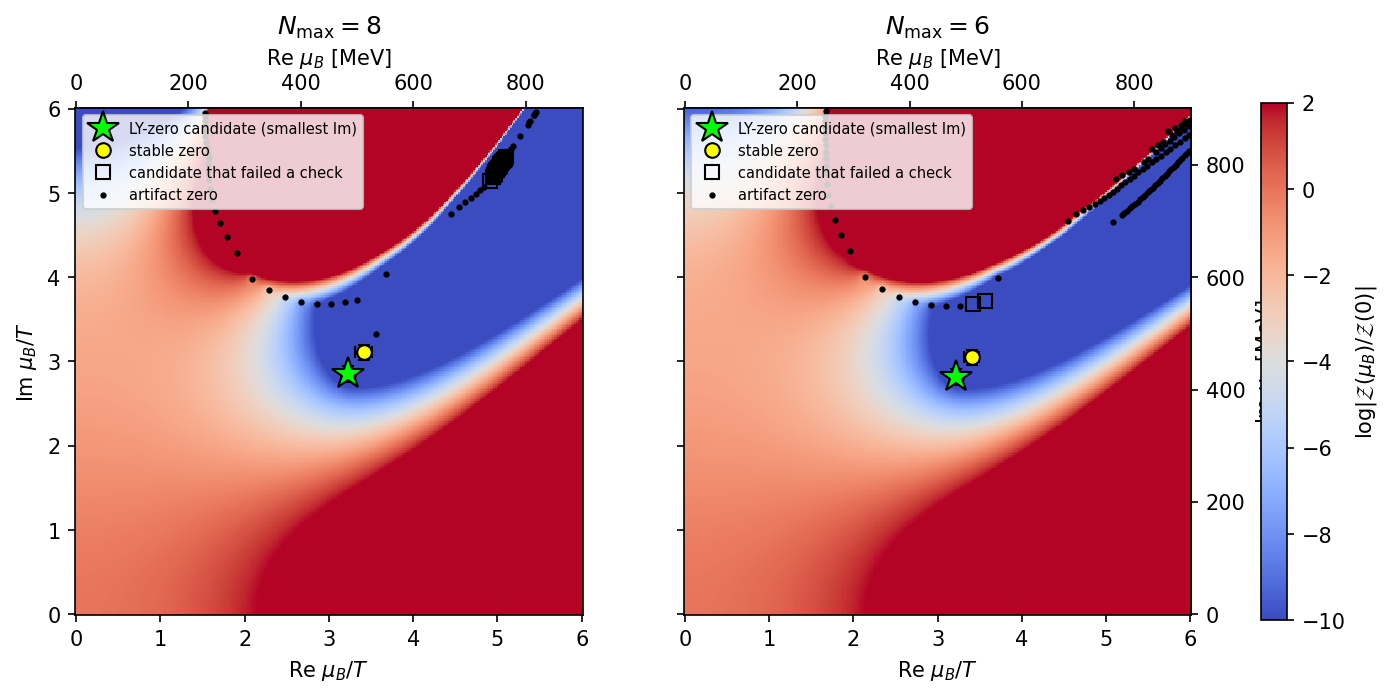
\includegraphics[width=\textwidth]{lee_yang.png}
\caption{$\log|Z(\muB)/Z(0)|$ at $T=150\MeV$ for $\Nmax=8$ (left) and 6 (right). Star: the candidate; yellow: stable zeros; dots: artifact zeros.}
\label{fig:heat}
\end{figure}

\section{Temperature scan (Taylor scheme)}

The leading zero is clean at 130--155\,MeV and moves towards the real axis as $T$ falls; the ends of the range fail for two different reasons. Table~\ref{tab:tscan} lists the candidate per temperature (\code{ly\_tscan.py}, errors stat $\oplus$ fit sys; the last column is the distance between the $\Nmax=8$ and 6 zeros, the truncation systematic).

\begin{table}[H]
\centering\small
\begin{tabular}{lllll}
\toprule
$T$ [MeV] & $\operatorname{Re}\mu_{LY}$ [MeV] ($N_8$ / $N_6$) & $\operatorname{Im}\mu_{LY}$ [MeV] ($N_8$ / $N_6$) & $|\mu_{LY}|/T$ ($N_8$) & $N_8$--$N_6$ distance [MeV] \\
\midrule
120 & no reliable zero & & & \\
125 & no reliable zero & & & \\
130 & 599(12) / 670(8) & 223(12) / 239(14) & 4.92 & 72 \\
135 & 565(10) / -- & 308(23) / -- & 4.77 & -- \\
140 & 539(14) / 571(12) & 337(14) / 317(15) & 4.54 & 37 \\
145 & 460(12) / 520(31) & 368(18) / 426(20) & 4.06 & 84 \\
150 & 484(12) / 483(12) & 428(14) / 423(14) & 4.31 & 5 \\
155 & 397(7) / 398(8) & 463(14) / 463(14) & 3.93 & 1 \\
160 & no isolated zero & & & \\
180 & no isolated zero & & & \\
\bottomrule
\end{tabular}
\caption{Leading Lee-Yang zero per temperature in the Taylor scheme.}
\label{tab:tscan}
\end{table}

At 120 and 125\,MeV the nearest $\Nmax=8$ zero has no $\Nmax=6$ partner within 2.5 in $\hmu$: the zero would sit at $|\hmu|\approx5.5$--7, where the $\hmu^8$ term controls the exponent. At 160 and 180\,MeV the nearest zeros form a row at $\operatorname{Im}\hmu\approx2.8$--$3.2\approx\pi$ with edge fractions near $10^{-3}$, the Roberge-Weiss-like structure of the model rather than an isolated zero. The candidate at 155\,MeV has $\operatorname{Im}\hmu=2.99\pm0.09$, close to $\pi$, which fits the same picture.

A Yang-Lee-edge fit $\operatorname{Im}\mu_{LY}=A\,(T-T_c)^{\beta\delta}$, $\beta\delta=1.5645$, on the five temperatures where both truncations agree (130, 140, 145, 150, 155) gives $T_c=87\pm4\MeV$ and $\operatorname{Re}\muB(T_c)=945\pm47\MeV$ at $\Nmax=8$ ($\chi^2/\mathrm{dof}=2.7/3$), and $T_c=83\pm5\MeV$, $\operatorname{Re}\muB=1176\pm61\MeV$ at $\Nmax=6$ ($\chi^2/\mathrm{dof}=7.6/3$). Dropping the lowest or highest temperature moves $T_c$ by at most 11\,MeV; the truncation systematic is 4\,MeV in $T_c$ and 230\,MeV in $\muB$, because the linear extrapolation of $\operatorname{Re}\mu_{LY}$ runs 45\,MeV past the data. For comparison, Fig.~5 of the notes (linear interpolation, $\Nmax=6$) has the $T=150\MeV$, $r=0$ zero near $(400$--$430)+400\,i\MeV$, read off the plot.

\begin{figure}[H]
\centering
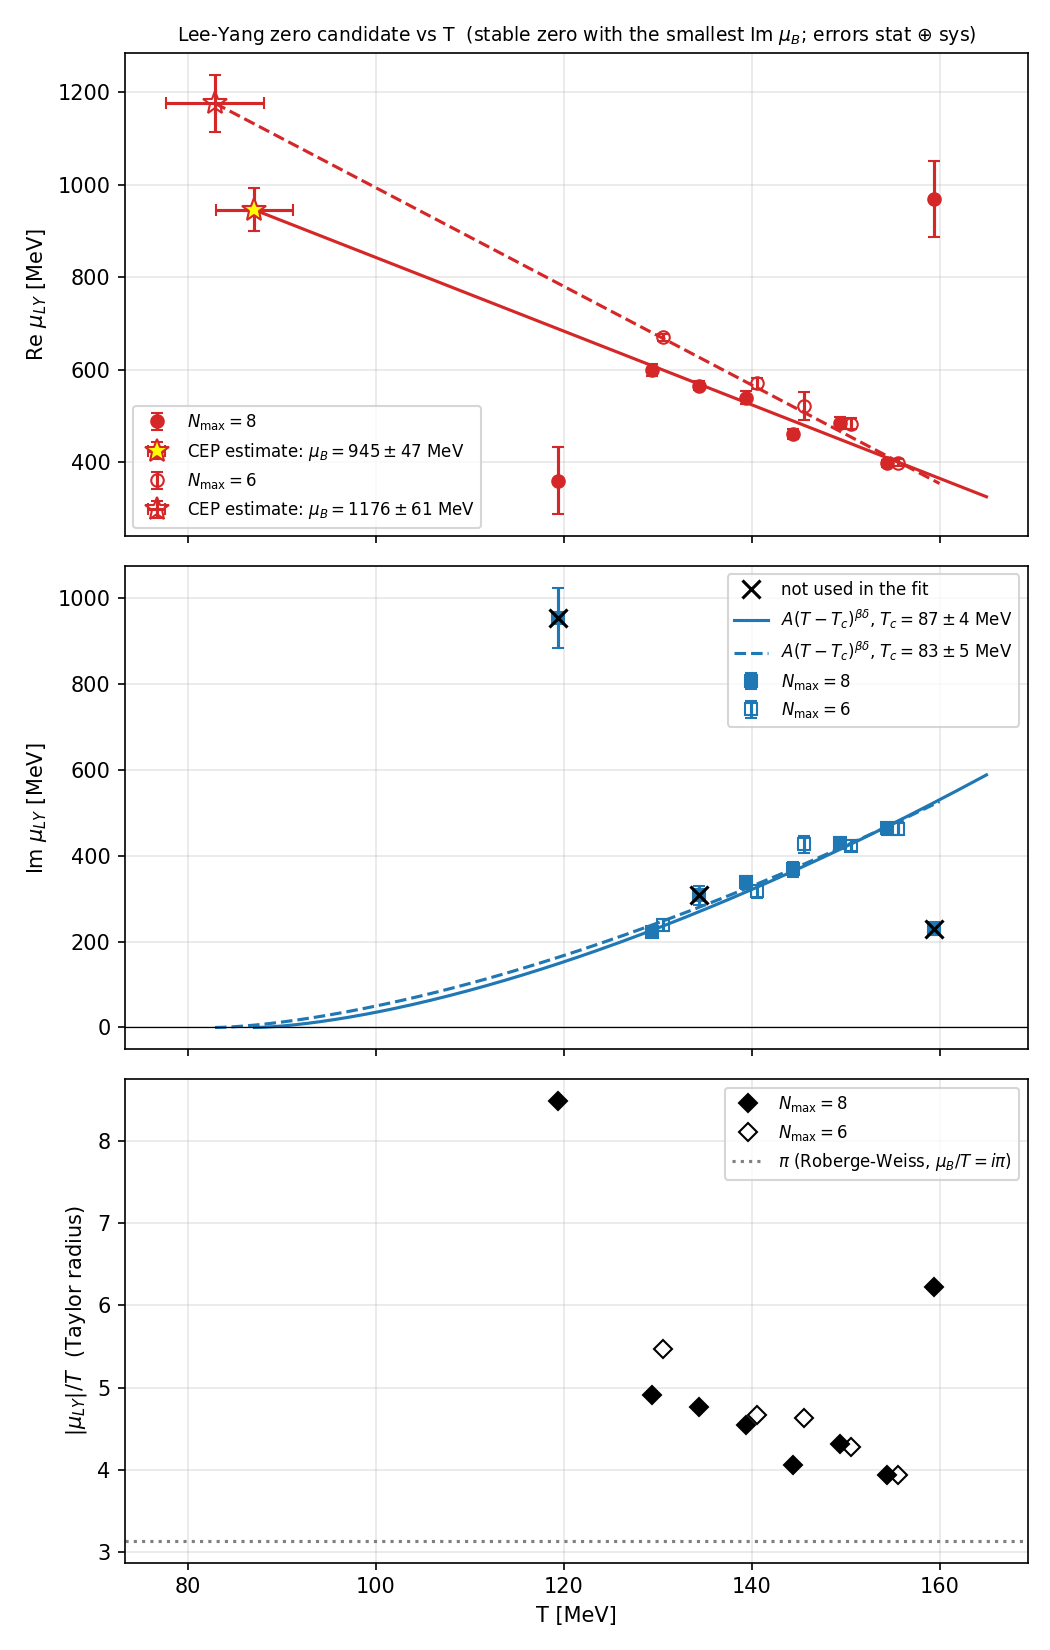
\includegraphics[width=0.78\textwidth]{ly_tscan.png}
\caption{Leading zero against $T$: real and imaginary parts in MeV with the Yang-Lee-edge fits, and the Taylor radius $|\mu_{LY}|/T$. Crosses mark temperatures excluded from the fit.}
\label{fig:tscan}
\end{figure}

\section{Scaling ans\"atze and the critical endpoint}

Four forms were fitted jointly to $\operatorname{Re}$ and $\operatorname{Im}\mu_{LY}(T)$ at 130, 140, 145, 150 and 155\,MeV with a shared $T_c$ (\code{ly\_scaling.py}), with point errors that include half the $\Nmax=8$ vs 6 distance. All agree that there is no critical point above about 125\,MeV; where they put it below that depends on the ansatz (Table~\ref{tab:scaling}, Fig.~\ref{fig:scaling}).

\begin{table}[H]
\centering\footnotesize
\begin{tabular}{lP{5.4cm}P{3.1cm}P{2.9cm}l}
\toprule
 & Ansatz & $T_c$ [MeV] ($N_8$ / $N_6$) & $\mu_c$ [MeV] ($N_8$ / $N_6$) & $\chi^2/\mathrm{dof}$ \\
\midrule
M1 & Ising edge: $\operatorname{Re}\mu=\mu_c+a(T-T_c)$, $\operatorname{Im}\mu=b(T-T_c)^{\beta\delta}$, $\beta\delta=1.5645$ & 81(10) / 80(7) & 1097(126) / 1223(94) & 10.7/6 \\
M2 & the same form in $z=\mu^2$ & $-139(68)$ / $-150(42)$ & 2093 / 2318 & 11.7/6 \\
M3 & M1 with a finite-volume floor, $\operatorname{Im}\mu=\sqrt{b^2(T-T_c)^{2\beta\delta}+f^2}$ & 81(16) / 80(12), $f=0$ & as M1 & 10.7/5 \\
M4 & M1 with a free exponent & 122(33) / 120(17), $\beta\delta=0.5(8)$ & 717(306) / 787(184) & 9.8/5 \\
\bottomrule
\end{tabular}
\caption{Scaling fits of the leading zero.}
\label{tab:scaling}
\end{table}

What the fits establish:
\begin{itemize}[nosep]
\item The joint Re\,+\,Im fit agrees with the Im-only fit (81 vs 87\,MeV); adding $\operatorname{Re}\mu_{LY}$ mostly fixes $\mu_c$.
\item The finite-volume floor comes out exactly zero. The Im data are concave in $T$ while a floor would make them convex, so with one volume there is no sign that the box holds the edge away from the real axis.
\item The exponent is not determined: $\beta\delta=0.5\pm0.8$ covers everything from linear to the Ising value, and $T_c$ slides to 120\,MeV with it. With five points 45--75\,MeV above $T_c$ the Ising exponent is an input, not a result.
\item The parametrisation matters more than the exponent: in $\mu^2$ the same Ising form extrapolates to $T_c<0$ because $\operatorname{Re}(\mu^2)=\operatorname{Re}^2-\operatorname{Im}^2$ falls steeply with $T$ in this range. The AIC cannot separate the two (weights 0.40 vs 0.23).
\end{itemize}
The defensible statement is a lower bound on $\mu_c$ of roughly 700\,MeV, not a location.

\begin{figure}[H]
\centering
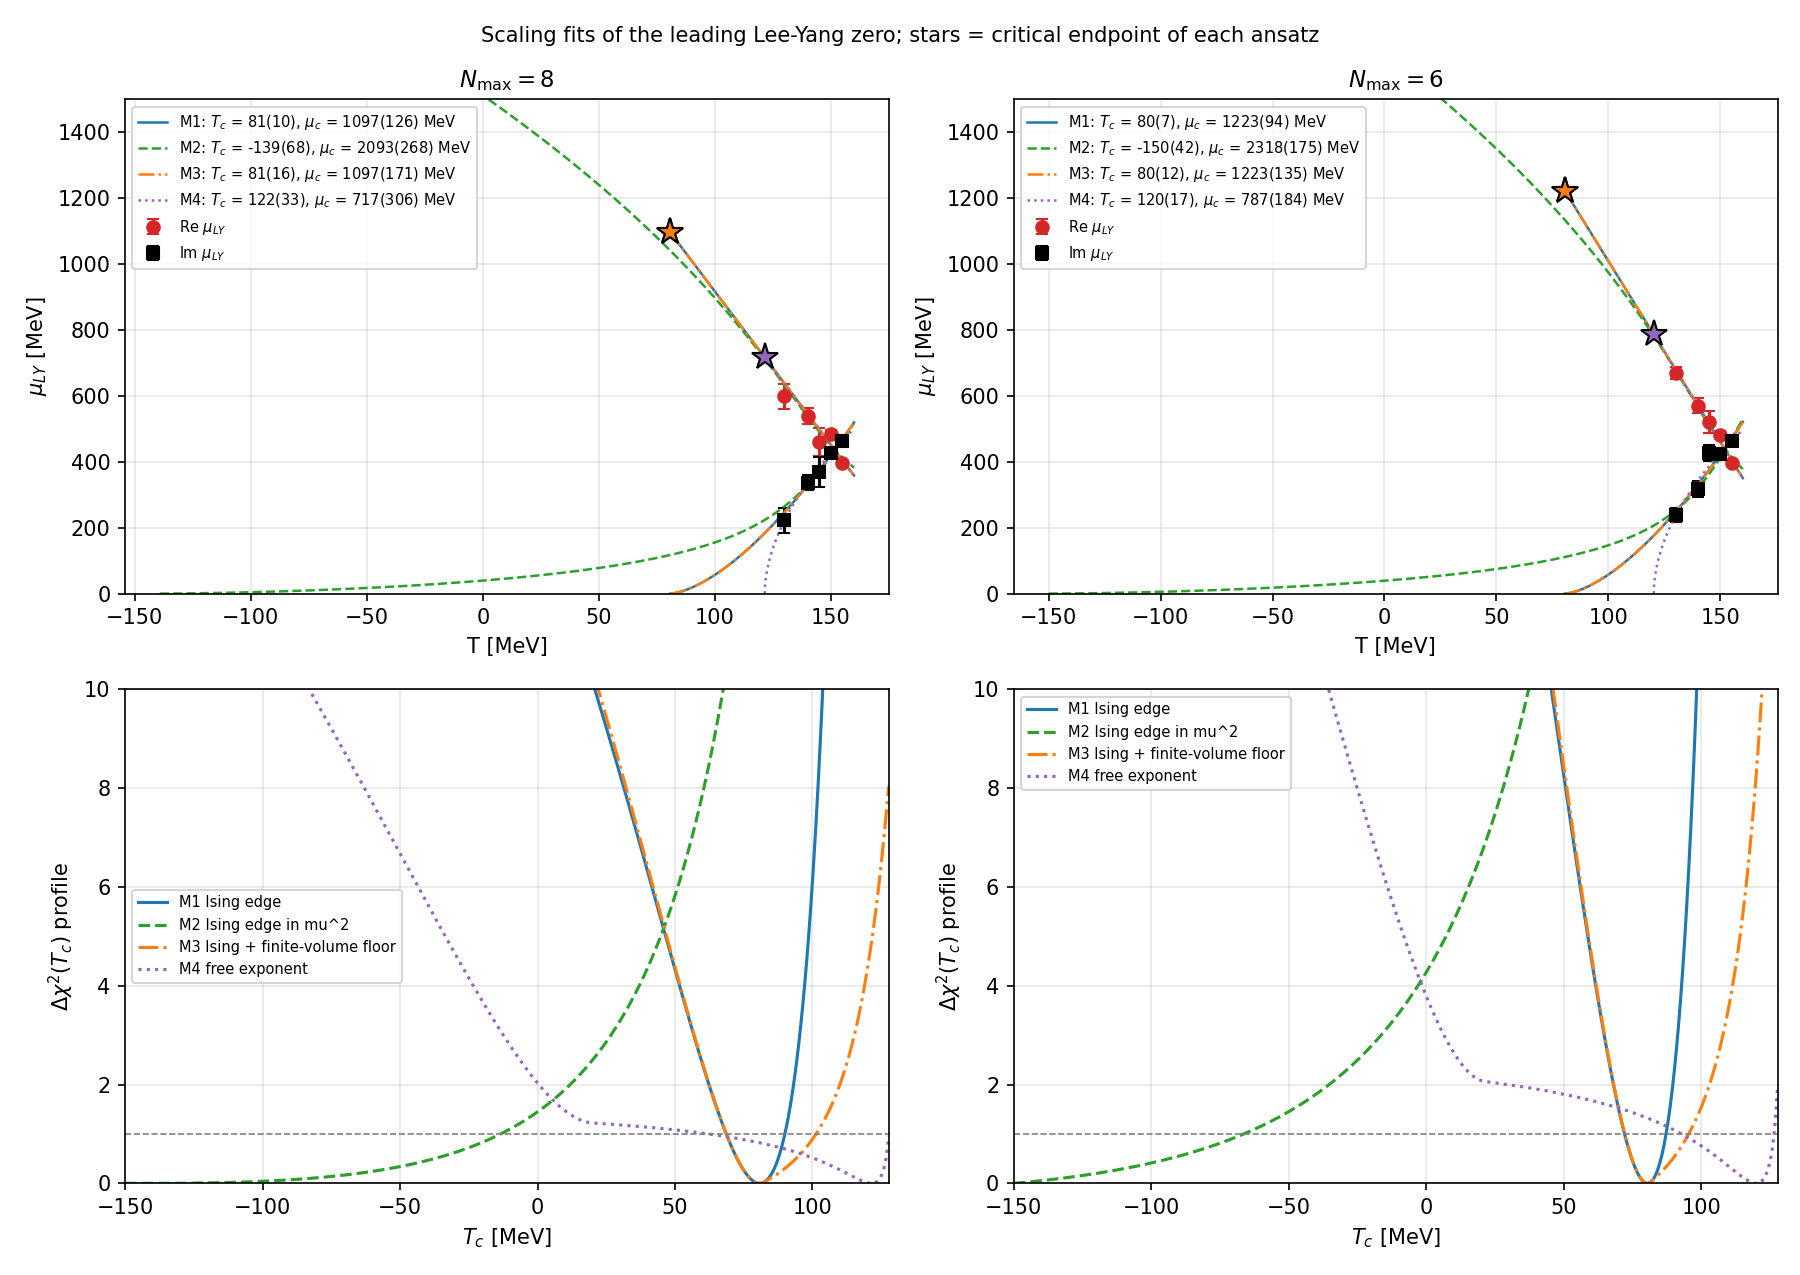
\includegraphics[width=\textwidth]{scaling_fit.png}
\caption{Scaling fits (top) and their $\Delta\chi^2$ profiles in $T_c$ (bottom), for $\Nmax=8$ (left) and 6 (right). Stars mark the critical endpoint of each ansatz.}
\label{fig:scaling}
\end{figure}

\section{Fugacity expansion}

Replacing the polynomial in $\hmu$ at fixed $c$ by baryon sectors, $\Delta\hat p(c)=\sum_B p_B(c)\,(\cosh(B\hmu)-1)$ with the $p_B$ matched to $\chi_2\ldots\chi_8$ (Eqs.~25--28 of the notes), restores the Roberge-Weiss periodicity but gives zeros whose position depends on how many sectors are kept. The scheme is a switch in the same code (\code{DOS\_SCHEME=fugacity}, \code{ly\_tscan.py -{}-scheme fugacity}).

Checks: the matching reproduces the notes' coefficients to $10^{-16}$ (e.g.\ $p_1=\tfrac{8}{5}\chi_2-\tfrac{61}{90}\chi_4+\tfrac{29}{360}\chi_6-\tfrac{1}{360}\chi_8$); the exponent is $2\pi$-periodic in $\operatorname{Im}\hmu$ and obeys $Z(-\hmu^*+2\pi i)=Z(\hmu)^*$ to machine precision; the fugacity and Taylor exponents agree to $7\cdot10^{-4}$ at $\hmu=1$ and diverge beyond. Because of the periodicity and the mirror symmetry, $\operatorname{Im}\hmu\in(0,\pi]$ is the whole fundamental domain, and beyond $\operatorname{Re}\hmu\approx3$ the highest sector's $e^{B\operatorname{Re}\hmu}$ makes the phase of $Z$ spin faster than any grid resolves, so the search is limited to $\operatorname{Re}\hmu\le6$ and the compared truncations are 2 and 1 sectors, as in Fig.~3 of the notes.

\begin{figure}[H]
\centering
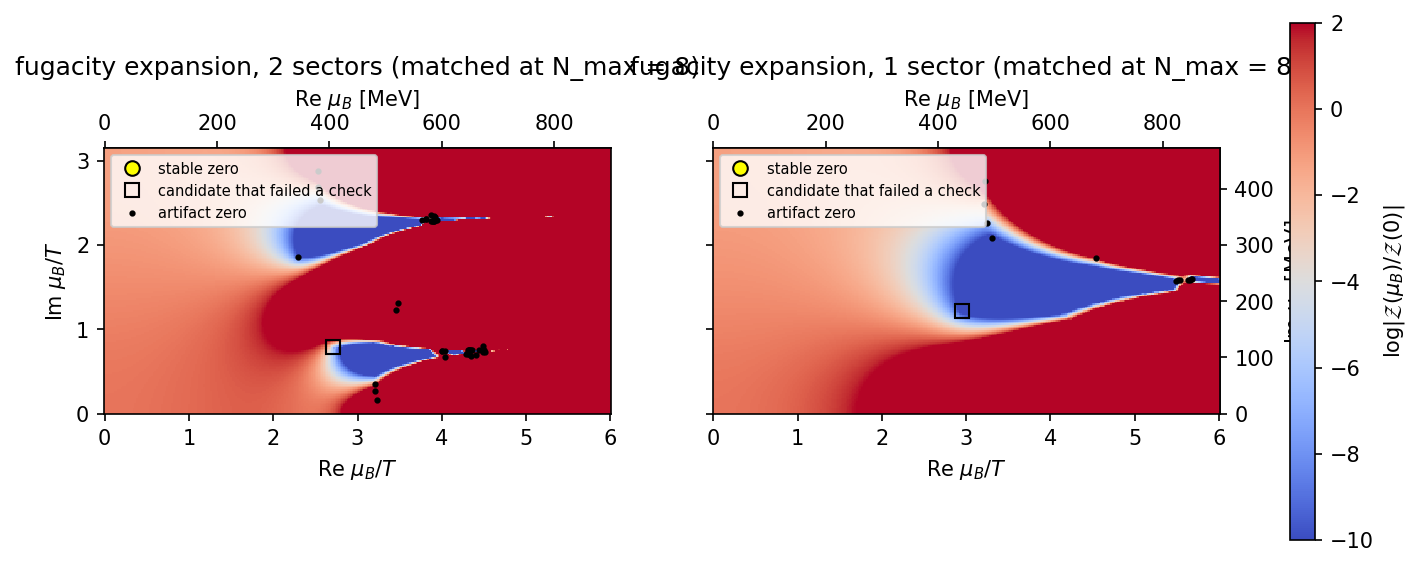
\includegraphics[width=\textwidth]{lee_yang_fugacity.png}
\caption{Fugacity scheme at $T=150\MeV$: 2 sectors (left) and 1 sector (right). One blue tongue per sector, mirrored at $\operatorname{Im}\hmu=\pi$.}
\label{fig:fug}
\end{figure}

Leading zero at $T=150\MeV$ by scheme and truncation:

\begin{center}\small
\begin{tabular}{lll}
\toprule
Scheme & Truncation & $\mu_{LY}$ [MeV] \\
\midrule
Taylor & $\Nmax=8$ & $484+428\,i$ \\
Taylor & $\Nmax=6$ & $483+423\,i$ \\
fugacity & 4 sectors & $369+264\,i$ \\
fugacity & 3 sectors & $346+311\,i$ \\
fugacity & 2 sectors & $407+118\,i$ \\
fugacity & 1 sector & $442+183\,i$ \\
\bottomrule
\end{tabular}
\end{center}

Across the scan the 2- and 1-sector zeros differ by 75--80\,MeV at every temperature except 180\,MeV, where $(420+392\,i)$ and $(469+342\,i)\MeV$ agree within the tolerance, so the stability filter rejects all other fugacity candidates and no CEP fit is possible in this scheme. The reason is structural: the $p_B$ are alternating combinations of the $\chi_n$ with large coefficients, and each sector carries $e^{B\operatorname{Re}\hmu}$, so adding or dropping a sector changes the integrand by factors of about 20 exactly where the zeros sit. This is the instability the notes report in Sec.~3.2.1, now with errors and across $T$. It also sets the scale of the scheme dependence that the Taylor $\Nmax$ comparison alone does not show: of order 100\,MeV for any zero with $|\hmu|\gtrsim3$.

\section{Lee-Yang zero ratio}

The ratio of the two leading zeros, $R_{21}=\operatorname{Im}z_2/\operatorname{Im}z_1$, is 1.03--1.14 at every usable temperature: the value expected when the zeros end at a Yang-Lee edge a finite distance from the real axis, not the 3 of a first-order transition. The method is from Wada, Kitazawa and Kanaya \cite{wada2025,kitazawa2025}: zeros are ordered by increasing imaginary part; for a first-order transition they are equally spaced, $\operatorname{Im}z_n\propto(2n-1)/V$, so $R_{21}\to3$; with no transition $R_{21}\to1$; at a critical point it takes a universal value independent of the volume, so curves for different $L$ cross there.

\begin{center}\small
\begin{tabular}{llll}
\toprule
$T$ [MeV] & $R_{21}$ ($N_8$) & $R_{21}$ ($N_6$) & $|z_2-z_1|$ in $\hmu$ \\
\midrule
130 & 1.10(8) & 1.14(8) & 0.28--0.31 \\
140 & 1.10(6) & 1.13(8) & 0.27--0.37 \\
145 & 1.04(7) & -- & 0.24 \\
150 & -- & 1.08(5) & 0.29 \\
155 & 1.04(5) & 1.04(5) & 0.17 \\
160 & 1.03(9) & -- & 0.26 \\
\bottomrule
\end{tabular}
\end{center}

The ratio in the even variable, $\operatorname{Im}(z_2^2)/\operatorname{Im}(z_1^2)$, gives the same picture (1.06--1.19). Entries are missing where one of the two zeros failed a stability check; there the ``second zero'' is a different object and the ratio scatters up to 2.2. With one volume this is a consistency check rather than a measurement: the crossing analysis that locates a critical point needs at least two $L$, and the spacing $\Delta\hmu\approx0.25$ is set by the width of $\rho_0$ and the slopes of $B_n(c)$, not by $2\pi/(\hV\,\Delta n_B)$, so the equal-spacing formula should not be read literally.

\begin{figure}[H]
\centering
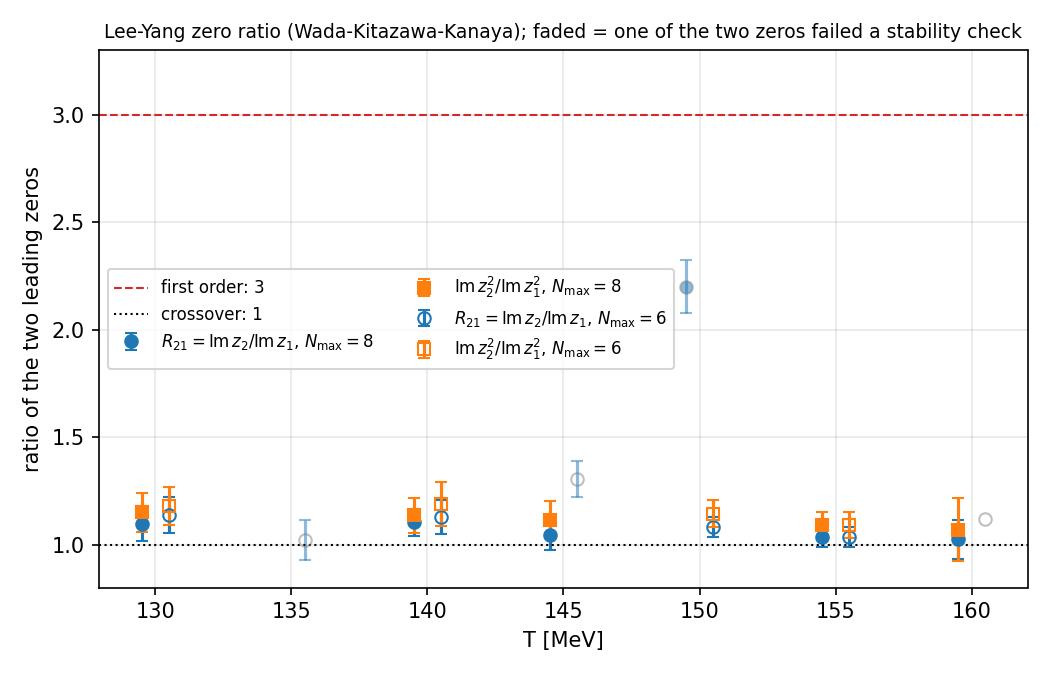
\includegraphics[width=0.8\textwidth]{ly_ratio.png}
\caption{Lee-Yang zero ratio against $T$. Dashed: first-order value 3; dotted: crossover limit 1; faded points have one of the two zeros failing a stability check.}
\label{fig:ratio}
\end{figure}

\section{Caveats and next steps}

The results are for one volume ($16^3$), one lattice spacing ($N_t=8$) and $\mu_S=0$, and the $\chi_n(c)$ enter through fits whose systematic is dominated by a single AIC variant. Beyond that:
\begin{itemize}[nosep]
\item The model cannot have zeros on the imaginary axis, so Roberge-Weiss periodicity is absent in the Taylor scheme by construction; the fugacity scheme has it but no stable zeros.
\item Any zero at $|\hmu|\gtrsim3$ carries a scheme dependence of order 100\,MeV (Taylor vs fugacity) that the $\Nmax=6$ vs 8 comparison does not show.
\item The CEP extrapolation depends on the ansatz ($\mu$ vs $\mu^2$, exponent fixed or free) more than on the data; 120 and 125\,MeV, where the zero would be most constraining, are not usable with $\Nmax=8$.
\item The stability filter is tuned by hand (tolerances 0.6, 0.15, 0.3 in $\hmu$, 10\% outliers); the values are listed in \code{lee\_yang.py} and every rejected zero is kept in the output with the reason.
\end{itemize}

What would sharpen the picture, in order of leverage:
\begin{enumerate}[nosep]
\item A second volume ($12^3\times8$ or $20^3\times10$ exist in the parent folder on katinka): it makes the finite-volume floor measurable and the zero-ratio crossing analysis possible.
\item The Polyakov-loop crossover line $T_c(\muB)$ and its curvature $\kappa_2$ from $\langle c\rangle_\mu(T)$ at real $\hmu\le2.5$, well inside the radius of convergence; the same machinery, ten temperatures, and a direct comparison with published values ($\kappa_2\approx0.012$--0.016).
\item The $\chi^{BS}_{nm}$ data on katinka for $\mu_S=r\muB$, including strangeness neutrality.
\item A linear-interpolation variant of the inner $c$ dependence, as in the notes, as a method systematic for the fit.
\end{enumerate}

\section{Files and how to rerun}

Everything lives in \code{\~{}/Desktop/Lattice\_QCD/Code/DoS/Playing\_around/}. The scripts need Python with numpy and matplotlib (\code{python3 -m pip install -{}-user numpy matplotlib}).

\begin{table}[H]
\centering\footnotesize
\begin{tabular}{P{4.7cm}P{5.8cm}P{4.5cm}}
\toprule
File & What it is & Rerun \\
\midrule
\code{raw/<T>/R.dat}, \code{B2.dat} \dots \code{B8.dat} & raw data copied from \code{katinka:/data/4hex/ana\_dos/16x8/<T>/} & -- \\
\code{dos\_common.py} & data loading, polynomial fits on jackknife samples, AIC variants, both expansion schemes & imported by the others \\
\code{chi\_calc.py} & $\chi^B_1\ldots\chi^B_8(\hmu)$ at $T=150$ $\to$ \code{chi\_calc.dat}, \code{.png} & \code{python3 chi\_calc.py} \\
\code{rho\_mu.py} & $\rho(c,\hmu)$, $\langle c\rangle$, $p$, $n_B$ at $T=150$ $\to$ \code{rho\_mu.dat}, \code{thermo\_mu.dat}, \code{.png} & \code{python3 rho\_mu.py} \\
\code{lee\_yang.py} & zero finder for one data set $\to$ \code{lee\_yang.dat}, \code{.png} & \code{DOS\_RAW=raw/150 DOS\_T=150 python3 lee\_yang.py} \\
\code{ly\_tscan.py} & runs \code{lee\_yang.py} for every $T$, collects candidates, CEP fit $\to$ \code{tscan/summary.dat}, \code{tscan/ly\_tscan.png}, \code{tscan/<T>/} & \code{python3 ly\_tscan.py [-{}-rerun] [-{}-scheme fugacity]} \\
\code{ly\_scaling.py} & the four scaling ans\"atze $\to$ \code{tscan/scaling\_fit.dat}, \code{.png} & \code{python3 ly\_scaling.py} \\
\code{ly\_ratio.py} & zero ratio $R_{21}$ $\to$ \code{tscan/ly\_ratio.dat}, \code{.png} & \code{python3 ly\_ratio.py} \\
\code{plot.py} & plots the old \code{.fit} files from the Desktop copy & \code{python3 plot.py} \\
\code{tscan\_fugacity/} & the same scan outputs for the fugacity scheme & -- \\
\code{notes/dos\_lee\_yang\_notes.tex} & this document & \code{tectonic dos\_lee\_yang\_notes.tex} \\
\bottomrule
\end{tabular}
\caption{Scripts and outputs.}
\end{table}

Without \code{-{}-rerun}, \code{ly\_tscan.py} reuses finished \code{tscan/<T>/lee\_yang.dat} files and only redoes the collection and the fit, which takes seconds; a full rerun is about one minute per temperature, four in parallel. Per-temperature logs with every zero and the check it failed are in \code{tscan/<T>/log.txt}.

\begin{thebibliography}{9}
\bibitem{notes} \emph{Yang-Lee edge singularity structure beyond standard lattice algorithms}, Fulbright research notes (DoS\_Notes-1.pdf), 28 October 2026.
\bibitem{wada2025} T.~Wada, M.~Kitazawa, K.~Kanaya, \emph{Finite-size scaling of Lee-Yang zeros and its application to the 3-state Potts model and heavy-quark QCD}, \href{https://arxiv.org/abs/2501.18904}{arXiv:2501.18904}.
\bibitem{kitazawa2025} M.~Kitazawa et al., \emph{Lee-Yang zeros in heavy-quark QCD}, \href{https://arxiv.org/abs/2503.22246}{arXiv:2503.22246}.
\bibitem{adam2025} A.~Adam et al., \emph{High-precision baryon number cumulants from lattice QCD in a finite box: cumulant ratios, Lee-Yang zeros and critical endpoint predictions}, \href{https://arxiv.org/abs/2507.13254}{arXiv:2507.13254}.
\end{thebibliography}

\end{document}
